\documentclass[14pt]{article}
\usepackage{../../report-tex/styles}


\begin{document}

    \titlewithlabnum{4}

    \tableofcontents
    \newpage


    \section{Мета:}
    Мета роботи – отримати вміння та навички проектування класів, виконавши модернізацію коду графічного редактора в об’єктно- орієнтованому стилі для забезпечення зручного додавання нових типів об'єктів.


    \section{Завдання:}
    1. Створити у середовищі MS Visual Studio C++ проект Win32 з ім’ям Lab4.\\
    2. Написати вихідний текст програми згідно варіанту завдання.\\
    3. Скомпілювати вихідний текст і отримати виконуваний файл програми.\\
    4. Перевірити роботу програми. Налагодити програму.\\
    5. Проаналізувати та прокоментувати результати та вихідний текст програми.\\
    6. Оформити звіт.\\

    \subsection{Варіант: }
    Варіанти завдань та основні вимоги\\
    1. Для усіх варіантів завдань необхідно дотримуватися вимог та положень, викладених вище у порядку виконання роботи та методичних рекомендаціях.\\
    2. Номер варіанту завдання дорівнює номеру зі списку студентів у журналі.\\

    \begin{align}
        &\text{Номер варіанту} = 22
    \end{align}\\
    Студенти з непарним номером (1, 3, 5, . . .) програмують глобальний статичний об'єкт класу MyEditor.\\
    Студенти з парним номером (2, 4, 6, . . .) програмують динамічний обєкт класу MyEditor, забезпечивши коректне його створення та знищення.\\
    3. Усі кольори та стилі (за винятком "гумового" сліду) геометричних форм – як у попередній лабораторній роботі No3. "Гумовий" слід при вводі усіх фігур малювати пунктирною лінією. \\
    4. Окрім чотирьох типів фігур, які були у попередніх лаб. No2 та 3, запрограмувати ще введення та відображення двох нових фігур – лінія з кружечками та каркас куба. Кольори ліній та заповнення цих нових фігур студент визначає на свій розсуд.\\
    Для об’єктів типів лінії з кружечками та каркасу кубу відповідні класи запрограмувати саме множинним успадкуванням. У цій лабораторній роботі не дозволяється замінювати множинне спадкування, наприклад, композицією. У першу чергу це стосується метода Show для нових фігур – для відображення ліній треба використовувати виклики метода Show з класу LineShape, для відображення кружечків – виклики метода Show з класу EllipseShape, а для відображення прямокутників – виклики метода Show з класу RectShape.\\
    5. Для усіх шости типів форм зробити кнопки Toolbar з підказками (tooltips)\\
    6. У звіті повинна бути схема успадкування класів – діаграма класів.\\
    Потрібно побудувати діаграму класів засобами Visual Studio C++.\\


    \section{Текст програми:}
    \subsection{Module: com.github.erotourtes.drawing.editor}
\lstinputlistingukr{DmProcessor.kt}{../src/main/kotlin/com/github/erotourtes/drawing/editor/DmProcessor.kt}
\lstinputlistingukr{Editor.kt}{../src/main/kotlin/com/github/erotourtes/drawing/editor/Editor.kt}
\lstinputlistingukr{Editors.kt}{../src/main/kotlin/com/github/erotourtes/drawing/editor/Editors.kt}
\lstinputlistingukr{ShapesList.kt}{../src/main/kotlin/com/github/erotourtes/drawing/editor/ShapesList.kt}

\subsection{Module: 1.0}
\lstinputlistingukr{MANIFEST.MF}{../src/main/resources/META-INF/MANIFEST.MF}

\subsection{Module: com.github.erotourtes.view}
\lstinputlistingukr{MainController.kt}{../src/main/kotlin/com/github/erotourtes/view/MainController.kt}
\lstinputlistingukr{MainView.kt}{../src/main/kotlin/com/github/erotourtes/view/MainView.kt}
\lstinputlistingukr{MenuBar.kt}{../src/main/kotlin/com/github/erotourtes/view/MenuBar.kt}
\lstinputlistingukr{ToolBar.kt}{../src/main/kotlin/com/github/erotourtes/view/ToolBar.kt}

\subsection{Module: com.github.erotourtes.app}
\lstinputlistingukr{MyApp.kt}{../src/main/kotlin/com/github/erotourtes/app/MyApp.kt}

\subsection{Module: com.github.erotourtes.drawing}
\lstinputlistingukr{CanvasPane.kt}{../src/main/kotlin/com/github/erotourtes/drawing/CanvasPane.kt}
\lstinputlistingukr{EditorHandler.kt}{../src/main/kotlin/com/github/erotourtes/drawing/EditorHandler.kt}

\subsection{Module: com.github.erotourtes.drawing.shape}
\lstinputlistingukr{Shape.kt}{../src/main/kotlin/com/github/erotourtes/drawing/shape/Shape.kt}
\lstinputlistingukr{Shapes.kt}{../src/main/kotlin/com/github/erotourtes/drawing/shape/Shapes.kt}

\subsection{Module: com.github.erotourtes.styles}
\lstinputlistingukr{ToolbarStyles.kt}{../src/main/kotlin/com/github/erotourtes/styles/ToolbarStyles.kt}

\subsection{Module: com.github.erotourtes.utils}
\lstinputlistingukr{Dimension.kt}{../src/main/kotlin/com/github/erotourtes/utils/Dimension.kt}
\lstinputlistingukr{ExtensionFunctions.kt}{../src/main/kotlin/com/github/erotourtes/utils/ExtensionFunctions.kt}
\lstinputlistingukr{Utils.kt}{../src/main/kotlin/com/github/erotourtes/utils/Utils.kt}




    \section{Ілюстрації:}
    \begin{figure}[H]
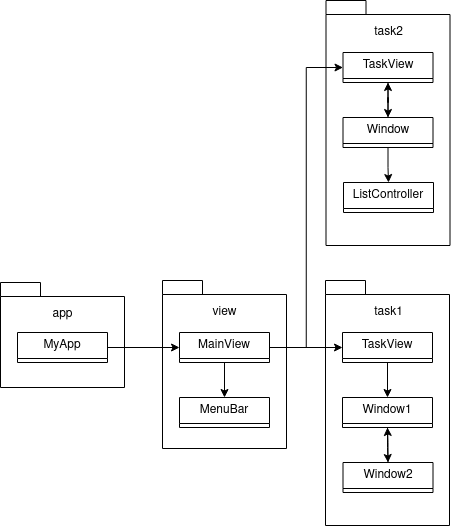
\includegraphics[width=10cm]{1}
\centering
\end{figure}



    \section{Висновки:}
    Отже, я отримав вміння та навички проектування класів, виконавши модернізацію коду графічного редактора в об’єктно- орієнтованому стилі для забезпечення зручного додавання нових типів об'єктів.
\end{document}
